\documentclass{article}
\usepackage[T1]{fontenc}
\usepackage{lmodern}
\usepackage{graphicx}
\usepackage{amsmath,amssymb}
\usepackage[a4paper,margin=2cm]{geometry}
\usepackage[absolute,overlay]{textpos}
\setlength{\TPHorizModule}{1mm}
\setlength{\TPVertModule}{1mm}
\usepackage[indonesian]{babel}
\usepackage{hyperref}
\setlength{\emergencystretch}{2em}
% unit: Halaman 16

\begin{document}

% === Halaman 16 (llm) ===

\begin{itemize}
    \item Pada awal enkripsi, 16-byte data masukan, $in_0, in_1, \dots, in_{15}$ disalin ke dalam array \texttt{state}, direalisasikan oleh fungsi:
    \[ \texttt{CopyPlaintextToState(state, plaintext)} \]
\end{itemize}

\vspace{60mm}

\begin{itemize}
    \item Pada akhir enkripsi, state disalin ke dalam \texttt{ciphertext}, direalisasikan oleh fungsi:
    \[ \texttt{CopyStateToCiphertext(ciphertext, state)} \]
\end{itemize}

% deskripsi: Diagram yang menunjukkan proses pemetaan data dari input bytes ke state array dan kemudian ke output bytes dalam bentuk matriks 4x4.
% bbox normalisasi: [0.1480, 0.2840, 0.8460, 0.6720]
\begin{textblock*}{146.58mm}(31.08mm,84.35mm)
\noindent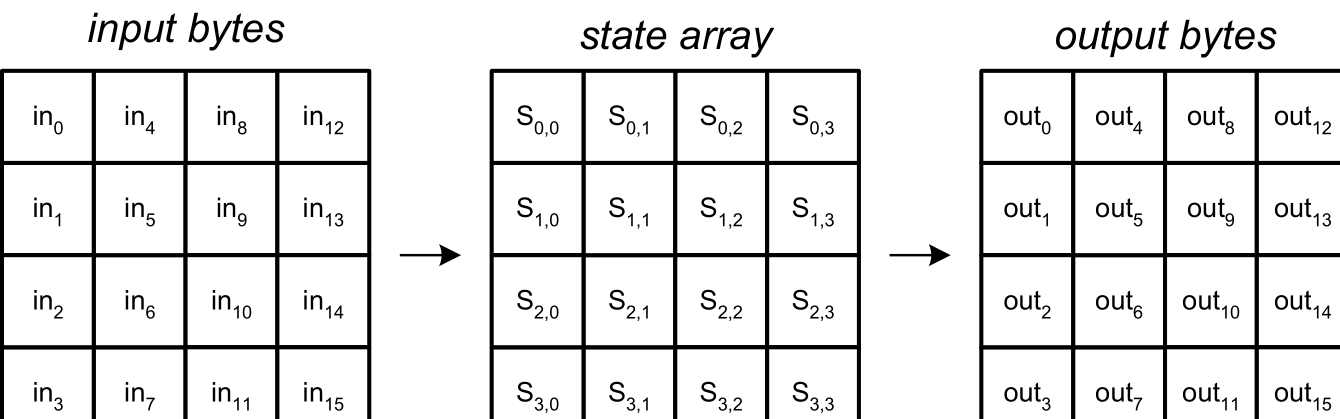
\includegraphics[width=146.58mm,height=115.24mm]{../../images/llm/page_016_img_01.png}%
\end{textblock*}

\end{document}
